\paragraph{Finding a preconditioning sequence}
To facilitate emotional conditioning I selected a specialized sequence containing images with a corresponding emotional charge.
Each sequence contains twenty-one to twenty-nine images with each displayed for a time of \textbf{five} seconds.

Each subject is assigned one of four preconditioning sequences. Each sequence is aimed to condition the subject into one of the 4 quadrants, described though a valence-arousal emotional model as mentioned in \ref{sec:emotion-theory}: Q1: angry, Q2: happy, Q3: sad, Q4: relaxed

There are several emotional image data-sets available for academic purposes such as GAPED \cite{Dan-Glauser2011}, OASIS \cite{Kurdi2017}, IAPS \cite{Lang1997} and NAPS \cite{Marchewka2014}. While NAPS is offering a high degree realism and quality of images, the range of it's images seems to cover "sad" and "happy" to a less pronounced degree. In general, strong negative valence values are accompanied with high arousal values across all analyzed data-sets. Causing sadness is a challenging task. In current preconditioning sequences I am using the \textbf{OASIS} database. It has comparatively wide spread of valence and arousal values compared to other sets.

\begin{figure}
	\centering
	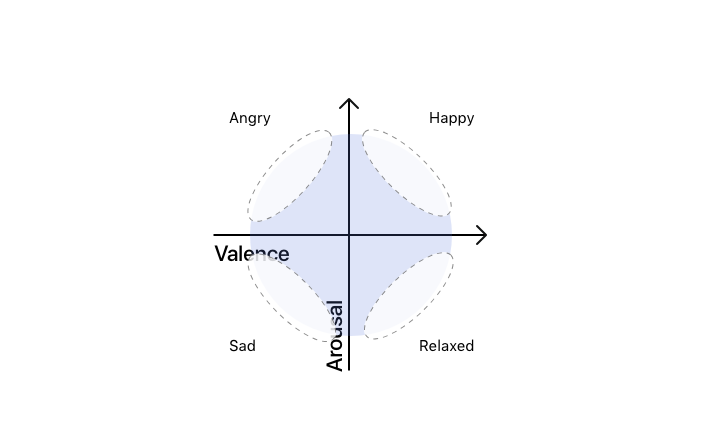
\includegraphics[width=0.7\linewidth]{graphics/Valence-Arousal-Model-1.png}
	\caption{Focus levels of emotional states on valence arousal model}
	\label{fig:valence-arousal-model-2}
\end{figure}

Keeping in mind the need for a clear separation between groups in terms of their emotional state into account, I limited emotional images to moderately strong stimuli values, thus avoiding extreme reactions and unrealistic emotional states. This limitation can limit the overall emotional effect of the preconditioning step on the participant. Figure \ref{fig:valence-arousal-model-2} highlights with dashed outline areas the target arousal and valence values, figure \ref{fig:allpreconditionings} illustrates all chosen images and their corresponding mean valence (x-axis) and arousal (y-axis). The scale of both axis is 1 to 7.

It can be assumed that in most cases, people who attend e-learning lessons will have moderate levels of emotional charge. It is important to note that quadrant 1 - angry and quadrant 2 - happy have a more pronounced representation in emotional databases due to an easier and more prevalent image stimuli availability. As such quadrant 1 and quadrant 2 have stronger stimuli compared to quadrant 3 and 4. The strength of effect is anticipated to be more strongly pronounced with participants who received the first and second quadrants.

It is expected that preconditioning sequence Q2 (high arousal, positive valence), which contains elements of erotic nature and features mostly women, will prove to be less effective in conditioning to Q2 of the Model of Affect with heterosexual female participants. Possibly even opposite results can be expected. Similar phenomenon has been observed in a cross-sexual comparison study of erotic subset for the Nencki Affective Picture System (NAPS, \cite{Wierzba2015}, where women participants rated female erotic images with significantly lower arousal and valence scores than heterosexual men. Due to the structure of the study it is not possible to determine the gender and sexual orientation of the participants before the preconditioning sequence is presented.






\begin{figure}[h!]
	\centering
	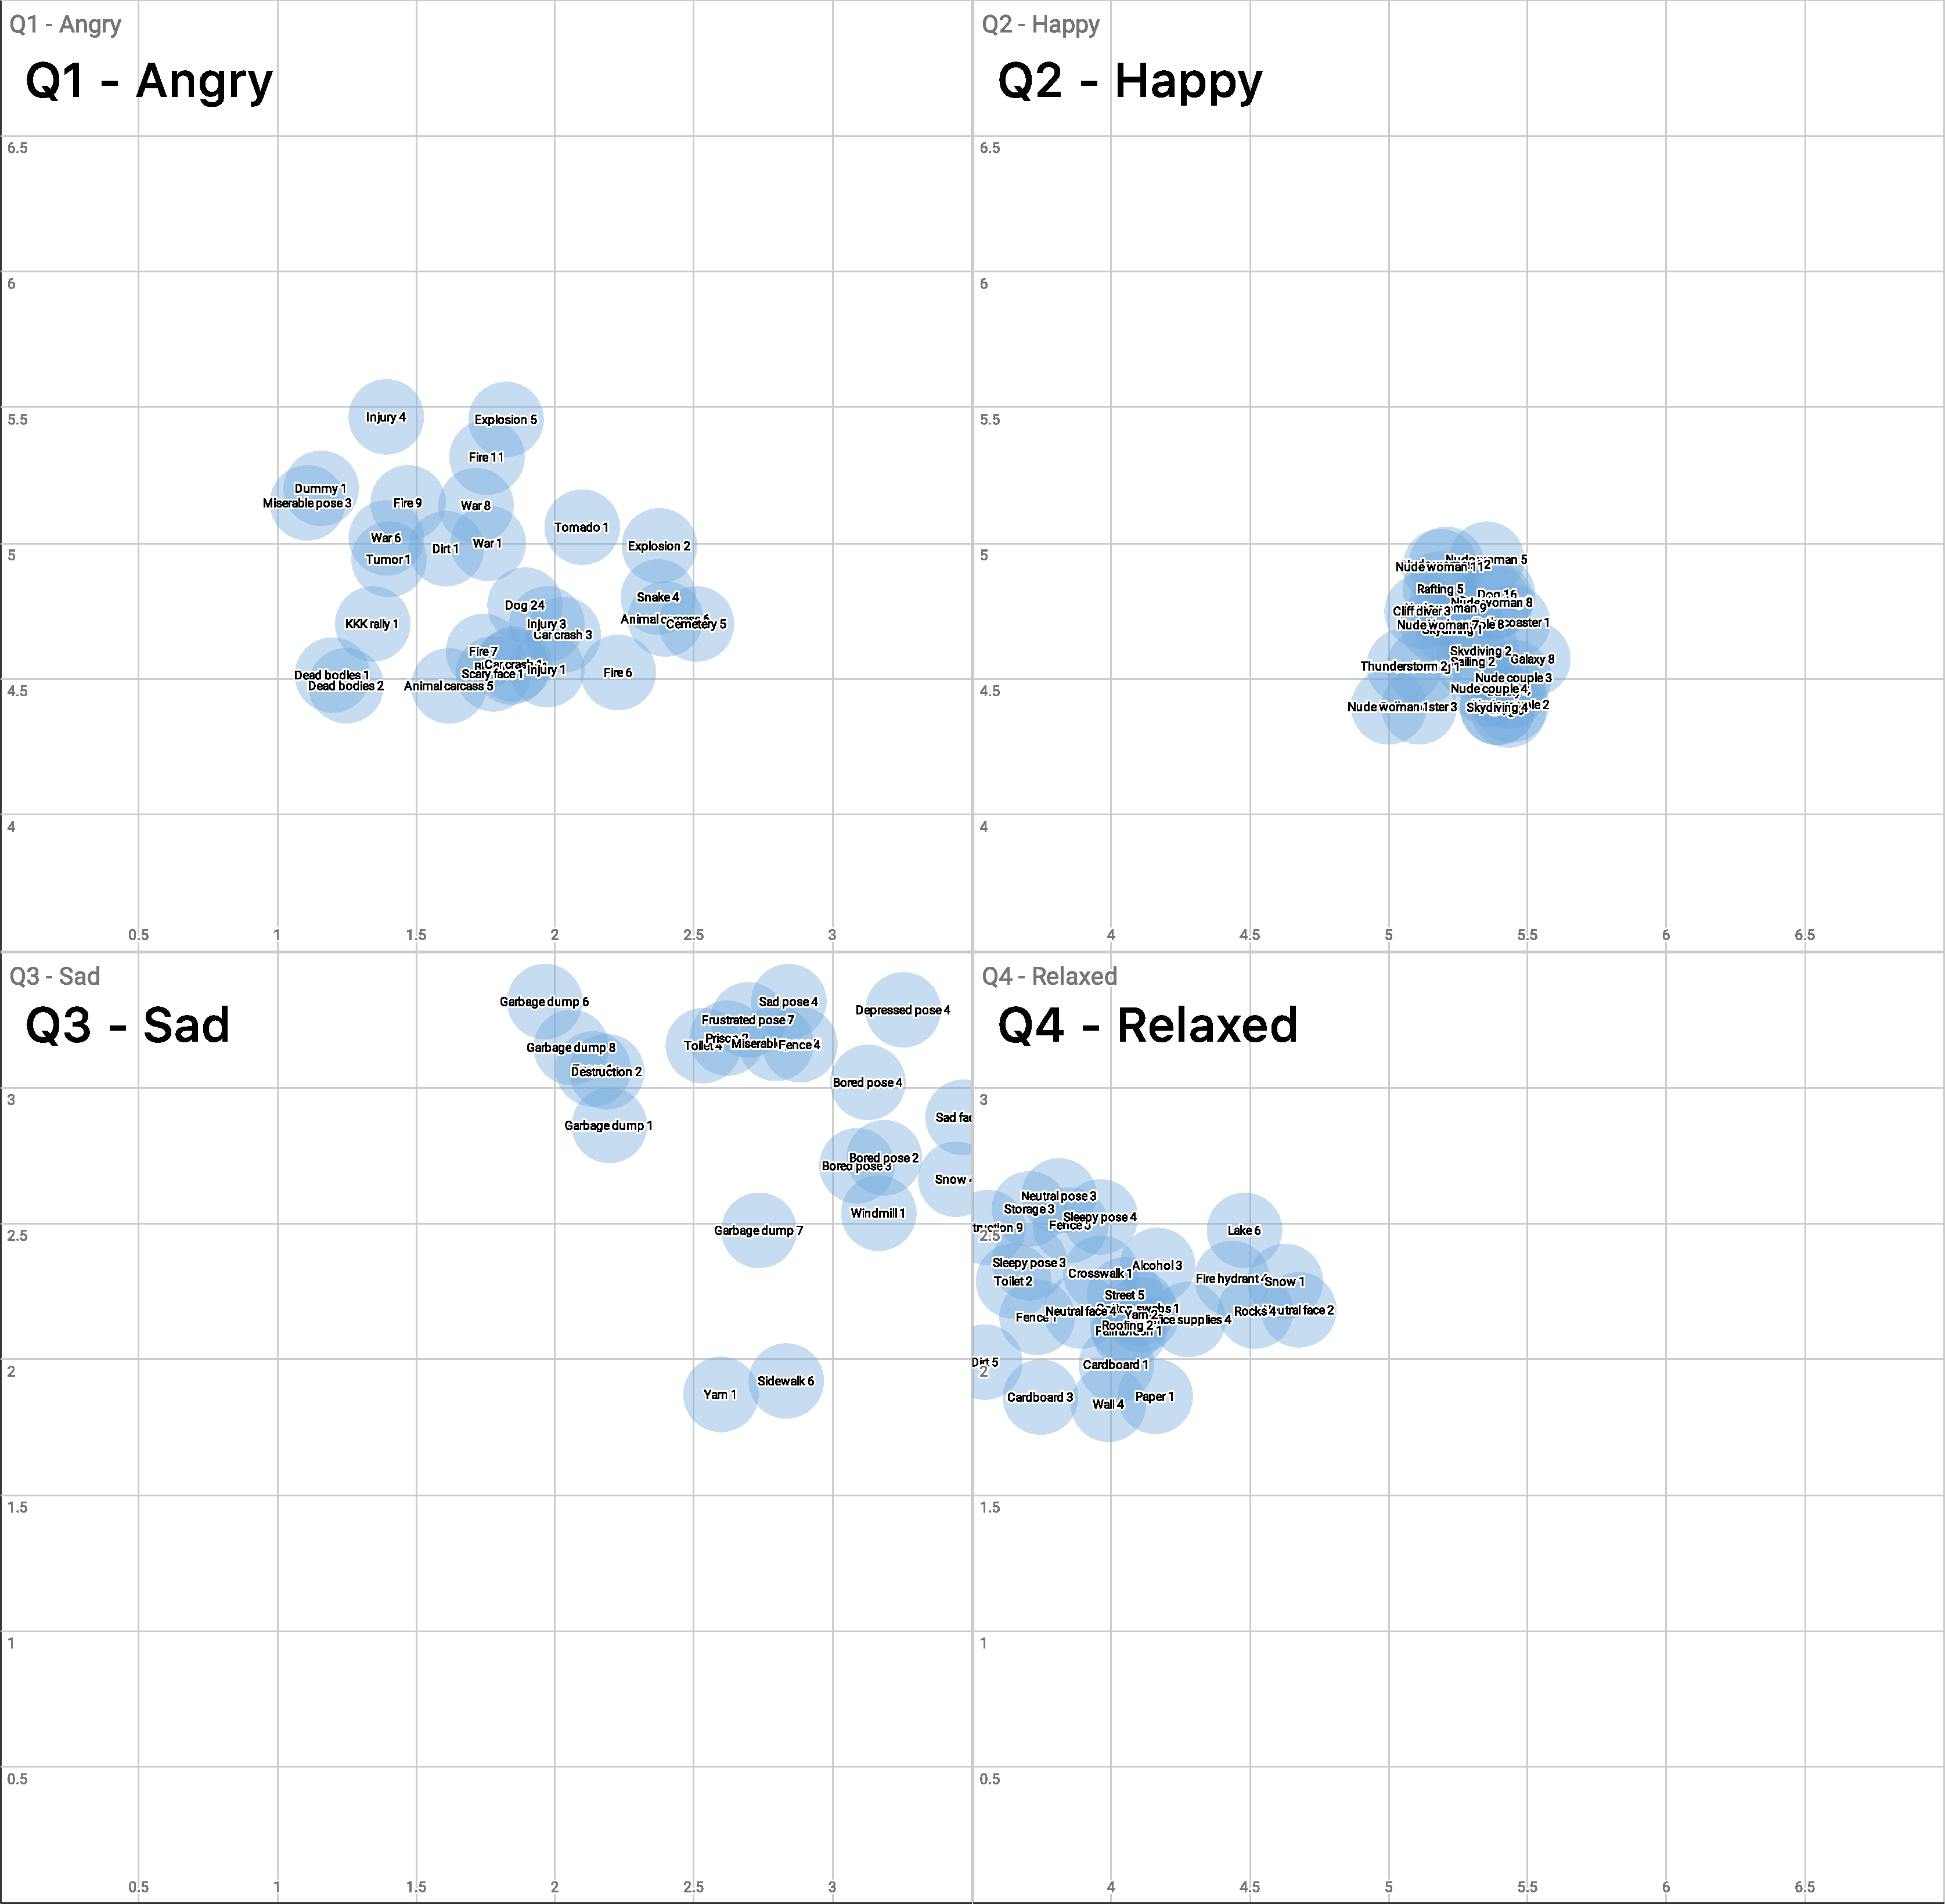
\includegraphics[width=1\linewidth]{graphics/All_Preconditionings}
	\caption{Chosen OASIS Preconditioning Images}
	\label{fig:allpreconditionings}
\end{figure}


\paragraph{Data:} Quadrants are mapped to preconditioning sequence encoding in data as follows \(Q(x) => Precond(x-1)\)